\documentclass[10pt,a4paper]{article}
\usepackage[utf8]{inputenc}
\usepackage{amsmath}
\usepackage{amsfonts}
\usepackage{amssymb}
\usepackage{amsthm}
\usepackage{float}
\usepackage{mathtools}
\usepackage{geometry}[margin=1in]
\usepackage{xspace}
\usepackage{tikz}
\usepackage{mathrsfs}
\usetikzlibrary{shapes, arrows, decorations.pathmorphing}
\usepackage[parfill]{parskip}
\usepackage{subcaption}
\usepackage{stmaryrd}
\usepackage{marvosym}
\usepackage{dsfont}

\newcommand{\st}{\text{ s.t. }}
\newcommand{\contr}{\lightning}
\newcommand{\im}{\mathfrak{i}}
\newcommand{\R}{\mathbb{R}}
\newcommand{\Q}{\mathbb{Q}}
\newcommand{\C}{\mathbb{C}}
\newcommand{\F}{\mathbb{F}}
\newcommand{\K}{\mathbb{K}}
\newcommand{\N}{\mathbb{N}}
\newcommand{\Z}{\mathbb{Z}}
\renewcommand{\H}{\mathds{H}}
\newcommand{\nequiv}{\not\equiv}
\newcommand{\powset}{\mathcal{P}}
\renewcommand{\th}[1][th]{\textsuperscript{#1}\xspace}
\newcommand{\from}{\leftarrow}
\newcommand{\legendre}[2]{\left(\frac{#1}{#2}\right)}
\newcommand{\ow}{\text{otherwise}}
\newcommand{\imp}[2]{\underline{\textit{#1.}$\implies$\textit{#2.}}}
\let\oldexists\exists
\renewcommand{\exists}{\oldexists\;}
\renewcommand{\hat}{\widehat}
\renewcommand{\tilde}{\widetilde}
\newcommand{\one}{\mathds{1}}
\newcommand{\under}{\backslash}
\newcommand{\injection}{\hookrightarrow}
\newcommand{\surjection}{\twoheadrightarrow}
\newcommand{\jacobi}{\legendre}
\newcommand{\floor}[1]{\lfloor #1 \rfloor}
\newcommand{\ceil}[1]{\lceil #1 \rceil}
\newcommand{\cbrt}[1]{\sqrt[3]{#1}}

\DeclareMathOperator{\ex}{ex}
\DeclareMathOperator{\id}{id}
\DeclareMathOperator{\upper}{Upper}
\DeclareMathOperator{\dom}{dom}

\DeclareMathOperator{\charr}{char}
\DeclareMathOperator{\Image}{im}
\DeclareMathOperator{\ord}{ord}
\DeclareMathOperator{\lcm}{lcm}
\let\emph\relax
\DeclareTextFontCommand{\emph}{\bfseries\em}

\newtheorem{theorem}{Theorem}[section]
\newtheorem{lemma}[theorem]{Lemma}
\newtheorem{corollary}[theorem]{Corollary}
\newtheorem{proposition}[theorem]{Proposition}
\newtheorem{conjecture}[theorem]{Conjecture}

\tikzset{sketch/.style={decorate,
 decoration={random steps, amplitude=1pt, segment length=5pt}, 
 line join=round, draw=black!80, very thick, fill=#1
}}

\title{Graph Theory}
\begin{document}
\maketitle
\section{Introduction}
\subsection*{Definitions}
Formally, we define a \emph{graph} to be an ordered pair $G = (V, E)$ where $E \subseteq V^{(2)} \coloneqq \{ Y \subseteq V : |Y| = 2\}$\\\\
e.g. $V = \{a,b,c,d\}, E = \left\{\{a,b\},\{a,c\},\{a,d\},\{b,c\}\right\}$\\
\begin{center}
\tikz{
\node (a) at (0,1) [circle, draw] {a};
\node (b) at (1,1) [circle, draw] {b};
\node (c) at (0,0) [circle, draw] {c};
\node (d) at (1,0) [circle, draw] {d};
\draw (a) edge (b) (a) edge (c) (a) edge (d) (b) edge (c);
}
\end{center}
The set \emph{$V(G)$} is the \emph{vertex set} of $G$ and \emph{$E(G)$} is the \emph{edge set}.\\
The \emph{order} of $G$ is $|V(G)|$, often written $|G|$.\\
The \emph{size} of G is $|E(G)|$, often written $e(G)$.\\
Note that for the purposes of this course, all graphs will be finite.

This definition that we use precludes:
\begin{itemize}
\item Having more than one edge between the same two vertices
\item Having an edge with both ends at the same vertex
\end{itemize}
\begin{figure}[h]
\begin{center}
\tikz{
\node (a) at (0,1) [circle,draw] {};
\node (b) at (1,1) [circle,draw] {};
\node (c) at (0.5,0.2) [circle,draw] {};
\node (d) at (1.5,0.5) [circle,draw] {};
\draw (a) edge[bend left] (b);
\draw (a) edge[bend right, red] (b);
\draw (a) edge (c);
\draw (b) edge (c);
\draw (c) edge (d);
\draw[red] (d.-60) arc (210:180+330:3mm);
}
\end{center}
\caption*{These 2 red edges are not allowed}
\end{figure}

Some authors allow graphs to have these features, and call what we're studying \emph{simple graphs}.

It's easier to write the edge $\{a,b\}$ as $ab$.\\
If $ab \in E(G)$, we say that ``$a$ is \emph{adjacent} to $b$'', and vice versa. We might write $ab \in G$.

Edges containing a vertex $x$ are said to be \emph{incident} to $x$ and to each other.

Two graphs $G, H$ are said to be \emph{isomorphic} if there exists a bijection\\ $f:V(G) \rightarrow V(H) \st uv\in E(G) \iff f(u)f(v) \in E(H)$.

There are some canonical graphs:

\begin{tabular}{c|c|c|c}
Name & Notation & Order & Size \\\hline
Empty graph & $E_n$ & $n$ & 0 \\
Complete graph & $K_n$ & $n$ & $\binom{n}{2}$ \\
Path & $P_n$ & $n$ & $n-1$ \\
Circuit & $C_n$ & $n$ & $n$
\end{tabular}\\
\begin{figure}
\begin{subfigure}{.3\textwidth}
\centering
\scalebox{1.5}{
\tikz{
\node (a) at (0,0.6) [circle, draw] {};
\node (b) at (0.6,1) [circle, draw] {};
\node (c) at (1.2,0.6) [circle, draw] {};
\node (d) at (0.9,0) [circle, draw] {};
\node (e) at (0.3,0) [circle, draw] {};
\draw (a) edge (b) edge (c) edge (d) edge (e);
\draw (b) edge (c) edge (d) edge (e);
\draw (c) edge (d) edge (e);
\draw (d) edge (e);
}}
\caption{$K_5$}
\end{subfigure}
\begin{subfigure}{.3\textwidth}
\centering
\scalebox{1.5}{
\tikz{
\node (a) at (0,0.5) [circle, draw] {};
\node (b) at (1,0) [circle, draw] {};
\node (c) at (2,0.5) [circle, draw] {};
\node (d) at (3,0) [circle, draw] {};
\draw (a) edge (b) (b) edge (c) (c) edge (d);
}}
\caption{$P_4$}
\end{subfigure}
\begin{subfigure}{.3\textwidth}
\centering
\scalebox{1.5}{
\tikz{
\node (a) at (0.2,0.5) [circle, draw] {};
\node (b) at (0.5,1) [circle, draw] {};
\node (c) at (1,1) [circle, draw] {};
\node (d) at (1.3,0.5) [circle, draw] {};
\node (e) at (1,0) [circle, draw] {};
\node (f) at (0.5,0) [circle, draw] {};
\draw (a) edge (b) (b) edge (c) (c) edge (d) (d) edge (e) (e) edge (f) (f) edge (a);
}}
\caption{$C_6$}
\end{subfigure}
\end{figure}

A \emph{subgraph} of $G$ is another graph $H$ with $V(H) \subseteq V(G), E(H) \subseteq E(G)$. (Ever graph of order $\leq n$ is a subgraph of $K_n$).\\
The subgraph of G \emph{induced by} $W \subseteq V(G)$, written $G[W]$ is the graph $(W, E(G)\cap W^{(2)})$, i.e. the vertex set $W$ and all edges of $G$ lying inside $W$.

A graph is \emph{connected} if there is a $u-v$ path (a path from $u$ to $v$ in $G$ for every pair $u,v \in V(G)$.\\
The \emph{components} of $G$ are the maximal connected subgraphs of $G$ (induced by the equivalence classes of the relation $u\leftrightarrow v \iff u = v$ or there is a $u-v$ path).

E.g.:\\
\tikz{
\node (a) at (0,0) [circle, draw] {};
\node (b) at (0.5,1) [circle, draw] {};
\node (c) at (1,0) [circle, draw] {};
\node (d) at (1.5,1) [circle, draw] {};
\node (e) at (2.5,1) [circle, draw] {};
\node (f) at (2,0) [circle, draw] {};
\node (g) at (3,1) [circle, draw] {};
\node (h) at (4,0) [circle, draw] {};
\node (i) at (5,0.5) [circle, draw] {};
\draw (a) edge (b) edge (c) (b) edge (c);
\draw (d) edge (e) (e) edge (f);
\draw (g) edge (h);
}\\
has 4 components.

A \emph{forest} is a graph containing no circuit.\\
A \emph{tree} is a connected forest, i.e. the components of a forest are trees.\\
Equivalently, a tree is a connected circuit-free graph. This bring us on to our first theorem of the course:

\begin{theorem}
The following are equivalent:
\begin{enumerate}
\item $G$ is a tree
\item $G$ is a minimal connected (connected, but the removal of any edge kills connectivity)
\item $G$ is maximal circuit-free (the addition of any edge creates a circuit)
\end{enumerate}
\end{theorem}

\begin{proof}
\subsubsection*{$(a) \implies (b)$}
Let $G$ be connected and circuit free. Suppose $uv\in G$ and $G-uv$ is connected. Then there is a $u-v$ path $P$ in $G-uv$, so $G$ contains the circuit $P+uv$ \contr ($G$ circuit free)\\
\therefore $G$ is minimal connected.
\subsubsection*{$(b) \implies (a)$}
Let $G$ be minimal connected, but suppose $G$ has a circuit $C$, with $xy \in C$. Let $u, v \in V(G)$. There is a $u-v$ path $P$ in $G$.\\
If $xy \notin P$, then $P$ joins $u$ to $v$ in $G-xy$.\\
If $xy \in P$, then $(P\cup C)-xy$ contains a $u-v$ path in $G-xy$.\\
Hence $G-xy$ is connected \contr ($G$ \emph{minimal} connected).\\
\therefore $G$ is circuit free, and connected by hypothesis, hence a tree.
\subsubsection*{$(a) \implies (c)$}
Let $G$ be a tree. If $uv \notin E(G)$ there is a path $P$ in $G$ from $u$ to $v$, so $P+uv$ is circuit in $G+uv$, so $G$ is maximal circuit free.
\subsubsection*{$(c) \implies (a)$}
Let $G$ be maximal circuit free. Let $u,v \in V(G)$. Either $uv \in E(G)$ or $G+uv$ has a circuit $C$, so $C-uv$ is a $u-v$ path in $G$, and so $G$ is connected, and hence a tree.
\end{proof}

A subgraph $T$ of a graph $G$ is said to be \emph{spanning} if $V(T) = V(G)$, i.e. the subgraph touches every vertex of $G$
\begin{corollary}
A graph is connected if and only if it has a spanning tree.
\end{corollary}
\begin{proof}
\item
\begin{itemize}
\item{$\implies$} $T$ is connected as it is a tree, and is spanning, so all vertices in $G$ are connected via $T$.
\item{$\Longleftarrow$} Remove edges from $G$ to obtain a minimal connected spanning subgraph $T$. By \textbf{1.1} $T$ is a tree.
\end{itemize}
\end{proof}

The set of \emph{neighbours} of a vertex $v$ is $\Gamma(v) = \{w: vw\in E(G)\}$.\\
The \emph{degree} $d(v)$ is the number of neighbours of $v$, $|\Gamma(v)|$\\
The minimum and maximum degrees in $G$ are denoted by $\delta(G)$ and $\Delta(G)$. \\
If $\delta(G) = \Delta(G) = k$, i.e. $d(v)=k \forall v$ we say $G$ is \emph{$k$-regular}. A \emph{regular} graph is one that is $k$-regular for some $k$. If a graph is $3$-regular, it is called \emph{cubic}.\\
The degrees of the graph written in some order form a \emph{degree sequence} of $G$.

\begin{lemma}[lemma Lemma]
\begin{align*}
\sum_{v\in G} d(v) = 2e(G)
\end{align*}
\end{lemma}
\begin{proof}
Each edge has $2$ vertices at the end, so contributes $2$ to the sum of all degrees.
\end{proof}
A \emph{leaf} is a vertex of degree $1$.
\begin{theorem}
Every tree $T$ with $|T|\geq 2$ has at least two leaves.
\end{theorem}
\begin{proof}
We note $T$ is connected so $\delta(T) \geq 1$. Let $x_1$ be a vertex (a leaf if there is one). Let $x_1x_2\ldots x_k$ be a maximal path from $x_1$. $T$ is circuit-free so none of $x_1,\ldots,x_{k-2}$ is in $\Gamma(x_k)$, and $x_k$ has no other neighbours except for $x_{k-1}$, otherwise this path can be extended, hence $\Gamma(x_k) = \{x_{k-1}\}$, so $x_k$ is a leaf. Repeat the proof starting at $x_k$ for a second leaf.
\end{proof}

\begin{corollary}
A tree of order $n$ has size $n-1$
\end{corollary}
\begin{proof}
\item
This is true for $n = 1, 2$ by inspection, as there is only 1 tree:

\begin{figure}[h]
\begin{subfigure}{.5\textwidth}
\centering
\tikz{
\node (a) at (0,0) [circle, draw] {};
}
\caption{$n=1$}
\end{subfigure}
\begin{subfigure}{.5\textwidth}
\centering
\tikz{
\node (a) at (0,0) [circle, draw] {};
\node (b) at (1,0) [circle, draw] {};
\draw (a) edge (b);
}
\caption{$n=2$}
\end{subfigure}
\end{figure}
Let $|T| \geq 3$. By \textbf{1.3} $T$ has a leaf $v$. Then $T-v$ is certainly circuit free and connected, because the $x-y$ path in $T$ uses $v$ if and only if $x$ or $y$ is $v$. Hence the corollary follows by induction.
\end{proof}

\begin{corollary}
The following are equivalent for a graph $G$ of order $n$:
\begin{enumerate}
\item $G$ is a tree
\item $G$ is connected and $e(G) = n-1$
\item $G$ is acyclic and $e(G) = n-1$
\end{enumerate}
\end{corollary}
\begin{proof}\item
\begin{itemize}
\item{$(1) \implies (2),(3)$:} True by definition and \textbf{1.5}.
\item{$(2) \implies (1)$:} By \textbf{1.2} $G$ contains a spanning tree $T$. By \textbf{1.5} $e(T) = e(G)$ so $T=G$
\item{$(3) \implies (1)$:} Add edges to $G$ to get a graph $G'$ maximal acyclic. By \textbf{1.1} $G'$ is a tree, so by \textbf{1.5} $e(G') = n-1 = e(G)$, so $G' = G$.
\end{itemize}
\end{proof}

\subsection*{How many graphs of order $n$ are there?}
Let the vertex set be $[n] \coloneqq \{1,2,\ldots,n\}$. E.g. for $n=3$  we have:\\
\begin{figure}[h]
\begin{subfigure}{0.12\textwidth}
\centering
\tikz{
\node (1) at (0,0) [circle, draw] {$1$};
\node (2) at (1,0) [circle, draw] {$2$};
\node (3) at (0.5,0.667) [circle, draw] {$3$};
}
\end{subfigure}
\begin{subfigure}{0.12\textwidth}
\centering
\tikz{
\node (1) at (0,0) [circle, draw, blue] {$1$};
\node (2) at (1,0) [circle, draw, blue] {$2$};
\node (3) at (0.5,0.667) [circle, draw, blue] {$3$};
\draw[blue] (1) edge (2);
}
\end{subfigure}
\begin{subfigure}{0.12\textwidth}
\centering
\tikz{
\node (1) at (0,0) [circle, draw, blue] {$1$};
\node (2) at (1,0) [circle, draw, blue] {$2$};
\node (3) at (0.5,0.667) [circle, draw, blue] {$3$};
\draw[blue] (1) edge (3);
}
\end{subfigure}
\begin{subfigure}{0.12\textwidth}
\centering
\tikz{
\node (1) at (0,0) [circle, draw, blue] {$1$};
\node (2) at (1,0) [circle, draw, blue] {$2$};
\node (3) at (0.5,0.667) [circle, draw, blue] {$3$};
\draw[blue] (2) edge (3);
}
\end{subfigure}
\begin{subfigure}{0.12\textwidth}
\centering
\tikz{
\node (1) at (0,0) [circle, draw, red] {$1$};
\node (2) at (1,0) [circle, draw, red] {$2$};
\node (3) at (0.5,0.667) [circle, draw, red] {$3$};
\draw[red] (2) edge (3);
\draw[red] (1) edge (2);
}
\end{subfigure}
\begin{subfigure}{0.12\textwidth}
\centering
\tikz{
\node (1) at (0,0) [circle, draw, red] {$1$};
\node (2) at (1,0) [circle, draw, red] {$2$};
\node (3) at (0.5,0.667) [circle, draw, red] {$3$};
\draw[red] (2) edge (3);
\draw[red] (1) edge (3);
}
\end{subfigure}
\begin{subfigure}{0.12\textwidth}
\centering
\tikz{
\node (1) at (0,0) [circle, draw, red] {$1$};
\node (2) at (1,0) [circle, draw, red] {$2$};
\node (3) at (0.5,0.667) [circle, draw, red] {$3$};
\draw[red] (1) edge (3);
\draw[red] (1) edge (2);
}
\end{subfigure}
\begin{subfigure}{0.12\textwidth}
\centering
\tikz{
\node (1) at (0,0) [circle, draw, green!70!black] {$1$};
\node (2) at (1,0) [circle, draw, green!70!black] {$2$};
\node (3) at (0.5,0.667) [circle, draw, green!70!black] {$3$};
\draw[green!70!black] (2) edge (3);
\draw[green!70!black] (1) edge (2);
\draw[green!70!black] (1) edge (3);
}
\end{subfigure}
\end{figure}\\
There are $2^{\binom{n}{2}}$ \emph{labelled} graphs of order $n$ - $\binom{n}{2}$ potentially edges, each of which we can independently choose to include or not.\\
However, there are only $4$ unlabelled graphs of order $3$ - all the graphs of the same colour are essentially the same, just with different labels given to the vertices. In general we must count the number of orbits amongst labelled graphs under the action of a group, using Burnside's Lemma. In fact, it turns out this number is asymptotic to $2^{\binom{n}{2}}/n!$

\subsection*{How many trees of order $n$ are there?}
\begin{theorem}[Cayley]
There are $n^{n-2}$ labelled tress of order $n$.
\end{theorem}
\begin{proof}(Pr\"ufer, Non-examinable)\\
We construct a bijection between trees strings length $n-2$ over the alphabet $n$.
\begin{itemize}
\item{\underline{Tree $\rightarrow$ string:}} Select the lowest leaf, write down its neighbour, remove that leaf, and repeat until only one edge is left.
\begin{center}
\tikz{
\node (1) at (5,2) [circle, draw] {$1$};
\node (2) at (6.5,2.3) [circle, draw] {$2$};
\node (3) at (5.1,1) [circle, draw] {$3$};
\node (4) at (6,0) [circle, draw] {$4$};
\node (5) at (3,1) [circle, draw] {$5$};
\node (6) at (8,2) [circle, draw] {$6$};
\node (7) at (1,2) [circle, draw] {$7$};
\node (8) at (6.1,1.5) [circle, draw] {$8$};
\node (9)  at (8,1) [circle, draw] {$9$};
\node (10) at (1,0.5) [circle, draw] {$10$};
\node (11) at (4,0.3) [circle, draw] {$11$};
\draw (1) edge (3);
\draw (2) edge (8);
\draw (3) edge (5) edge (8) edge (11);
\draw (4) edge (11);
\draw (5) edge (10) edge (7);
\draw (6) edge (8);
\draw (8) edge (9);
}
\end{center}
Here, we would get the string $3, 8, 11, 8, 5, 8, 3, 5, 10$. Each vertex is written down $d(n)-1$ times
\item{\underline{String $\rightarrow$ tree:}} Mark all vertices "unused". Then repeatedly choose the smallest unused vertex not in the string. Join it to the first vertex in the string. Mark it as used. Delete first vertex in the string.
\end{itemize}
\end{proof}

A graph is \emph{$r$-partite} if its vertices can be partitioned into $r$ classes so that no edge lies within a class. In the special case where $r=2$ we call the graph \emph{bipartite}. Remarkably, we can characterise all bipartite graphs.
\begin{theorem}
A graph is bipartite if and only if it contains no odd circuit.
\end{theorem}
\begin{proof}
For the ``only if" part, in a bipartite graph the vertices of a circuit alternate between the two classes, otherwise an edge would lie in a class. Hence any circuit must be of even length.

For the ``if" part, take some graph $G$, pick a vertex $v_0$ and let $V_i = \{v : d(v_0,v) = i\}$ where $d(v_0,v)$ is the \emph{distance} of $v$ from $v_0$, i.e. the length of a shortest $v_0-v$ path. 
\begin{center}
\tikz{
\node[circle, draw] (v0) at (0,0) {$v_0$};
\node[black!75!white, ellipse, draw, minimum width=0.3cm, minimum height=2cm] (v1) at (2,0) {$V_1$};
\node[black!50!white, ellipse, draw, minimum width=0.3cm, minimum height=2cm] (v2) at (4,0) {$V_2$};
\node[black!25!white, ellipse, draw, minimum width=0.3cm, minimum height=2cm] (v3) at (6,0) {$V_3$};
\node[ellipse, minimum width=0.3cm+15pt, minimum height=2cm] (v4) at (8,0) {};
\node (l) at (8,0) {$\cdots$};
\draw[black!88!white] (v0) edge (v1.110) edge (v1) edge (v1.250);
\draw[black!63!white] (v1.70) edge (v2.110) (v1.290) edge (v2.250) (v1) edge (v2);
\draw[black!38!white] (v2.70) edge (v3.110) (v2.290) edge (v3.250) (v2) edge (v3);
\draw[black!13!white] (v3.70) edge (v4.110) (v3.290) edge (v4.250) (v3) edge (v4);
}
\end{center}
If $G$ is connected, $V_0, V_1, V_2, \ldots$ partition $V(G)$. (Note $V_0 = \{v_0\}$). There is no edge between $V_i$ and $V_{i+k}$ if $k \geq 2$ by construction. Suppose $G$ has no odd circuit. Then $G$ cannot have an edge inside one of the $V_i$: if $u,v \in V_i$ and $uv\in G$, then there is a way of getting from $v_0$ to itself in an odd number of steps. $v_0 \xrightarrow{i} u \xrightarrow{1} v \xrightarrow{i} v_0$. This must contain an odd circuit: let the first path be $v_0=a_0,a_1,a_2,\ldots, a_{i-1}, u$ and the second be $v_0=b_0,b_1,b_2,\ldots,b_{i-1},v$, and let $k = \max\{j: a_j=b_j\}$, so $0\leq k <i$. Then $a_k, a_{k+1},\ldots,u,v,b_{i-1},\ldots,b_k=a_k$ is an odd cycle.  Hence we can let our two classes be $\cup_i V_{2i}$ and $\cup_i V_{2i+1}$, and $G$ is bipartite.
\end{proof}

An \emph{Euler cycle} as a ``walk" around all the edges of a graph returning to the starting point so that every vertex is visited and every edge is used precisely once.
\begin{figure}
\centering
\scalebox{0.8}{
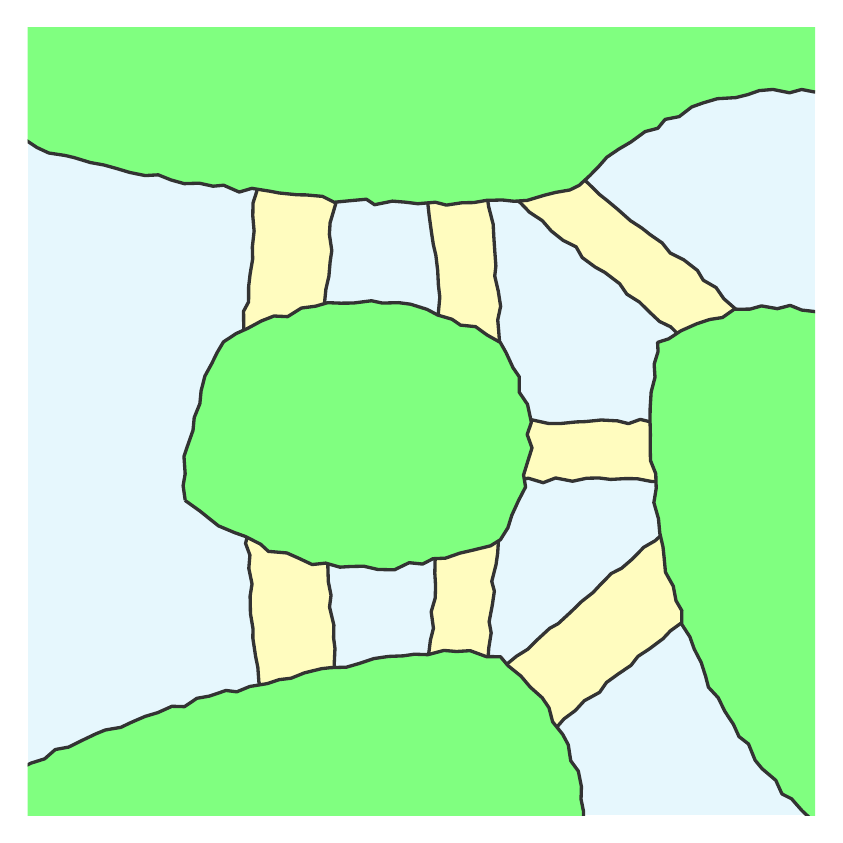
\begin{tikzpicture}

\clip [preaction={fill=cyan!10}] (0,0) rectangle (10,10);

\foreach \p/\r/\w/\h in 
  {(3,1)/5/1/4, (3,9)/-5/1/-4, (5,1)/-5/0.75/4, (5,9)/5/0.75/-4, 
  (5,5)/-90/0.75/4, (5,1)/-50/1/4, (6,8)/50/0.75/-4}
\draw [sketch=yellow!25]
   [shift={\p}, rotate=\r] rectangle +(\w,\h);

\draw [sketch=green!50]
  (-1,-1) -- (-1,0) to [bend left, looseness=0.5] (6,2) to [bend left] (7,-1) 
  (11,-1) to [bend left] (8,6) to [bend left] (11,6) -- cycle
  (-1,9) to [bend right, looseness=0.5] (7,8) to [bend left] 
  (11,9) -- (11,11) -- (-1,11) -- cycle
  (2,4) to [bend left, looseness=0.5] (2.5,6) to [bend left] 
  (6,6) to [bend left] (6,3.5) to [bend left] (2,4) -- cycle;
\end{tikzpicture}
}
\caption*{The bridges of K\"onigsberg, which inspired this problem}
\end{figure}

A graph is \emph{Eulerian} if it is a single vertex or has an Euler cycle.
\begin{theorem}
A graph is Eulerian if and only if it is connected and every vertex has even degree
\end{theorem}
\begin{proof}
The forwards direction is clear: an Eulerian graph must be connected, and for every time we enter a vertex along an edge we must also leave that vertex, so each vertex has even degree.

We do the opposite direction by induction on $e(G)$. Since $\delta(G) \geq 2$ by \textbf{1.4} $G$ is not a tree and so has a circuit $C$. Every vertex of $G-E(C)$ has even degree, so by induction each component of $G-E(C)$ is Eulerian. Now set off walking round $C$, taking the time to traverse any Euler cycle of $G-E(C)$ when first encountered. Since $G$ is connected, this gives an Euler cycle of $G$.
\end{proof}

A graph that can be drawn in the plane without edges crossing is \emph{planar}. A graph drawn in the plane is a \emph{plane graph}. A \emph{face} of a plane graph is a connected region of $\R^2\setminus G$. We define the \emph{size} of a face to be the number of edges it has.\\
E.g.:
\begin{figure}[h]
\begin{subfigure}{.5\textwidth}
\centering
\tikz{
\node (a) at (0,2) [circle, draw] {};
\node (b) at (1.5,0) [circle, draw] {};
\node (c) at (3,2) [circle, draw] {};
\node (d) at (4.5,0) [circle, draw] {};
\node (e) at (6,2) [circle, draw] {};
\draw (a) edge (b) edge (c) (b) edge (c) edge (d) (c) edge (d) edge (e) (d) edge (e);
}
\caption{Face sizes $3,3,3,5$}
\end{subfigure}
\begin{subfigure}{.5\textwidth}
\centering
\tikz{
\node (a) at (3,0.6) [circle, draw] {};
\node (b) at (1.5,0) [circle, draw] {};
\node (c) at (3,2) [circle, draw] {};
\node (d) at (4.5,0) [circle, draw] {};
\node (e) at (6,2) [circle, draw] {};
\draw (a) edge (b) edge (c) (b) edge (c) edge (d) (c) edge (d) edge (e) (d) edge (e);
}
\caption{Face sizes $3,3,4,4$}
\end{subfigure}
\end{figure}

These two graphs are the same planar graph, but are different plane graphs. Note that we include the outer infinite face. There are no analytical/topological difficulties involved. Any planar graph can be drawn with piecewise linear edges, and in fact with straight line edge (see example sheet 1), so any issues are purely combinatorial.

\begin{theorem}[Euler]
Let $G$ be a connected plane graph with $n$ vertices, $m$ edges, and $f$ faces. Then $n-m+f = 2$.
\end{theorem}
\begin{proof}
$G$ has a spanning tree with $n-1$ edges, so $m\geq n-1$. If $m=n-1$ then $G$ is a tree, in which case $f=1$ so done. We now proceed by induction on $m$. If $m>n-1$, there is a circuit $C$. If we remove an edge from this circuit, then we obtain a graph with 1 fewer edge and 1 fewer face, and so by the induction hypothesis, $n-(m-1)+(f-1)=2 \implies n-m+f=2$.
\end{proof}

A \emph{bridge} (or \emph{isthmus}) is an edge whose removal increases the number of components. Equivalently, it's an edge which is not part of any circuit. In a connected bridgeless plane graph, every edge separates two faces. So if there are $f_i$ faces of length $i$, then $\sum_i f_i = f$ and $\sum_i if_i = 2m$.

The \emph{girth} of a graph is the length of its shortest circuit.

\begin{theorem}
Let $G$ be a connected bridgeless planar graph of girth $g$, order $n$, size $m$. Then:
\begin{align*}
m\leq \frac{g}{g-2}(n-2)
\end{align*}
In particular, every planar graph of order $n\geq 3$ has size at most $3n-6$ and contains a vertex of degree $\leq 5$.
\end{theorem}
\begin{proof}
Draw $G$ in the plane, with $f_i$ faces of length $i$. Then $2n = \sum_i if_i \geq g\sum_i f_i = gf$. By \textbf{1.10}, $n-2=m-f \geq m-\frac{2}{g}m = m\frac{g-2}{g}$, establishing the claimed formula.

Now given any planar graph, add edges if necessary to make it connected and bridgeless. Since the girth $g\geq 3$, $m\leq 3n-6$. By the lemma lemma, the average degree is less than 6.
\end{proof}
\subsection*{Some Planar Graphs}
\begin{figure}[h]
\begin{subfigure}{.5\textwidth}
\centering
\tikz{
\node (a) at (0,0) [circle, draw] {};
\node (b) at (1,1.7) [circle, draw] {};
\node (c) at (2,0) [circle, draw] {};
\node (d) at (1,0.6) [circle, draw] {};
\draw (a) edge (b) edge (c) edge (d) (b) edge (c) edge (d) (c) edge (d);
}
\caption*{$K_4$ is planar}
\end{subfigure}
\begin{subfigure}{.5\textwidth}
\centering
\tikz{
\node (a) at (0.4,0) [circle, draw] {};
\node (b) at (0,1.2) [circle, draw] {};
\node (c) at (1,2) [circle, draw] {};
\node (d) at (2,1.2) [circle, draw] {};
\node (e) at (1.6,0) [circle, draw] {};
\draw (a) edge (b) edge (c) edge (d) edge (e) (b) edge (c) edge (d) edge (e) (c) edge (d) edge (e) (d) edge (e);
}
\caption*{$K_5$ is non-planar, as violates the $m\leq 3n-6$}
\end{subfigure}
\end{figure}
The \emph{complete bipartite} graph $K_{m,n}$ is bipartite with class sizes $m$ and $n$ and all edges between, so $|K_{m,n}| = m+n, e(K_{m,n}) = mn$, girth $=4$ if $m,n\geq 2$.
\begin{figure}[H]
\begin{subfigure}{.5\textwidth}
\centering
\tikz{
\node (a) at (0,1) [circle, draw] {};
\node (b) at (4,1) [circle, draw] {};
\node (c) at (2,2) [circle, draw] {};
\node (d) at (2,1.6) [circle, draw] {};
\node (e) at (2,1.2) [circle, draw] {};
\node (f) at (2,0.7) {$\vdots$};
\node (g) at (2,0) [circle, draw] {};
\draw (a) edge (c) edge (d) edge (e) edge (g) (b) edge (c) edge (d) edge (e) edge (g);
}
\caption*{$K_{2,n}$ is planar}
\end{subfigure}
\begin{subfigure}{.5\textwidth}
\centering
\tikz{
\node (a) at (0,0) [circle, draw] {};
\node (b) at (0,1) [circle, draw] {};
\node (c) at (0,2) [circle, draw] {};
\node (d) at (2,0) [circle, draw] {};
\node (e) at (2,1) [circle, draw] {};
\node (f) at (2,2) [circle, draw] {};
\draw (a) edge (d) edge (e) edge (f) (b) edge (d) edge (e) edge (f) (c) edge (d) edge (e) edge (f);
}
\caption*{$K_{3,3}$ is non-planar, as violates the $m\leq 3n-6$}
\end{subfigure}
\end{figure}

Any graph of order $n$ with more than $3n-6$ edges is non-planar but there are non-planar graphs with many fewer edges.\\
Take any graph $G$. A \emph{subdivision} or \emph{topological} $G$ is any graph obtained from $G$ by replacing its edges with paths whose internal vertices are disjoint. Any such subdivision is denoted by $TG$.

\begin{figure}[H]
\begin{subfigure}{.5\textwidth}
\centering
\tikz{
\node (a) at (0,0) [circle, draw] {};
\node (b) at (1,1.7) [circle, draw] {};
\node (c) at (2,0) [circle, draw] {};
\node (d) at (1,0.6) [circle, draw] {};
\draw (a) edge (b) edge (c) edge (d) (b) edge (c) edge (d) (c) edge (d);
}
\caption*{$G$}
\end{subfigure}
\begin{subfigure}{.5\textwidth}
\centering
\tikz{
\node (a) at (0,0) [circle, draw] {};
\node (a2) at (0.3333,0.5667) [circle, draw] {};
\node (a3) at (0.6667,1.1333) [circle, draw] {};
\node (b) at (1,1.7) [circle, draw] {};
\node (bd) at (1,1.15) [circle, draw] {};
\node (b2) at (1.4,1.02) [circle, draw] {};
\node (b3) at (1.6,0.68) [circle, draw] {};
\node (c) at (2,0) [circle, draw] {};
\node (d) at (1,0.6) [circle, draw] {};
\node (c1) at (0.4,0) [circle, draw] {};
\node (c2) at (0.8,0) [circle, draw] {};
\node (c3) at (1.2,0) [circle, draw] {};
\node (c4) at (1.6,0) [circle, draw] {};
\draw (a) edge (a2);
\draw (a2) edge (a3);
\draw (a3) edge (b);
\draw (a) edge (d);
\draw (b) edge (bd);
\draw (bd) edge (d);
\draw (b) edge (b2);
\draw (b2) edge (b3);
\draw (b3) edge (c);
\draw (c) edge (d);
\draw (a) edge (c1) (c1) edge (c2) (c2) edge (c3) (c3) edge (c4) (c4) edge (c);
}
\caption*{$TG$}
\end{subfigure}
\end{figure}
Kuratowski (1930) and Pontryagin (much earlier, unpublished) characterised planar graphs:
\begin{theorem}[Kuratowski]
$G$ is planar if and only if it contains no $TK_5$ and no $TK_{3,3}$.
\end{theorem}
We will not prove this here.

Given a plane graph, we can draw a new graph, the \emph{dual graph}, by placing a dual vertex inside each original face and adding a dual edge for every original edge separating the two faces. 

\begin{center}
\scalebox{0.8}{
\tikz{
\node[circle, fill=blue, draw] (a) at (0,0) {};
\node[circle, fill=blue, draw] (b) at (0,4) {};
\node[circle, fill=blue, draw] (c) at (3,4) {};
\node[circle, fill=blue, draw] (d) at (3,0) {};
\node[circle, fill=blue, draw] (e) at (5,2) {};
\node[circle, fill=orange, draw] (a*) at (1,3) {};
\node[circle, fill=orange, draw] (b*) at (2,1) {};
\node[circle, fill=orange, draw] (c*) at (3.8,2) {};
\node[circle, fill=orange, draw] (d*) at (2,6) {};
\draw (a) edge (b) edge (c) edge (d) (b) edge (c) (c) edge (d) (e) edge (c) edge (d);
\draw[dashed] (a*) edge (b*) edge (d*) edge[out=210, in=190, looseness=2.8] (d*) (b*) edge (c*) edge[out=250, in=180, looseness=4] (d*) (c*) edge[bend right=60] (d*) edge[out=-50, in=0, looseness=3.5] (d*);
}}
\end{center}
\vspace{-4cm}
If $G$ has $v$ vertices, $e$ edges, $f$ faces; dual of $G$ has $f$ vertices, $e$ edges, $v$ faces. The dual of the dual is the original graph. Note that, as seen in this example, we do allow there to be multiple edges between the same pair of vertices in the dual graph.

\section{Matchings and Connectivity}
Let $G$ be a bipartite graph with vertex classes $X, Y$. A \emph{matching} from $X$ to $Y$ is a set of $|X|$ independent edges (edges that are not incident).
\begin{center}
%ellipse with 3 points - X, larger ellipse - Y. Edges from each point to Y
\end{center}
If $|X| = |Y|$, such a matching is also a matching of $Y$ to $X$. We call it a \emph{1-factor} (i.e. a \emph{1-regular} spanning subgraph). We can think of this in terms of arranged marriages of things in $X$ and $Y$, but I'm not sure why you would. A matching from $X$ to $Y$ does not always exist (for instance, if $|X|>|Y|$), but remarkably, a simple necessary condition is also sufficient.

Firstly, given $A\subset V(G)$ define $\Gamma(A) = \cup_{a\in A}\Gamma(a)$. Then we can say:
\begin{theorem}[Hall's Marriage Theorem]
Let $G$ be a bipartite graph with bipartition $X, Y$. Then there is a matching from $X$ to $Y$ if and only if:
\begin{align*}
|\Gamma(A)| \geq |A| \; \forall \. A \subseteq X
\end{align*}
This condition is known as Hall's condition.
\end{theorem}
\begin{proof}
The ``only if" part is immediate. We will prove the ``if" part in several ways:

\underline{Proof 1:} \\
By induction on $|X|$.\\
Either for all $\emptyset \neq A \neq X$ the inequality $\Gamma(A)| > |A|$ holds. Let $xy$ be any edge. Then Hall's condition still holds in $G' = G-x-y$. Then by induction match $X-x$ to $Y-y$, which together with $xy$ gives a matching $X$ to $Y$.\\
Or there exists a ``critical set" $\emptyset \neq B \neq X$ with $|\Gamma(B)| = |B|$
\begin{center}
%Blob with UpLeft B; UR \Gamma(B); LL X-B; LR Y-\Gamma(B) dotted line through middle going horiz
\end{center}
Let $G_1 = G[B \cup \Gamma(B)], G_2 = G[(X\setminus B)\cup (Y \setminus \Gamma(B))]$. Let $A \subset B$, then $\Gamma(A) \subset \Gamma(B)$. Since Hall's condition holds in $G$ it holds in $G_1$. Let $A \subset X \setminus B$. Then $\Gamma_2(A) \coloneqq \Gamma(A\cup B) \setminus \Gamma(B)$, so $|\Gamma_2(A)| = |\Gamma(A\cup B)| - |\Gamma(B)| \geq |A\cup B| - |B|$ since $|\Gamma(B)| = |B|$. So Hall's condition holds in $G_1$ and $G_2$.

\underline{Proof 2} (Rado):
Remove edges to get a minimal graph where Hall's Condition holds. If $d(a)=1$ for all $a\in X$, then what's left is a matching. If not, then some $a\in X$ has two neighbours $b_1, b_2$ and sets $A_1, A_2$ such that $|\Gamma(A_i)| = |A_i|$, and $\Gamma(a)-b_i \subset \Gamma(A_i)$. So $|\Gamma(A_1 \cup A_2 \cup \{a\}) = \Gamma(A_1\cup A_2)$, and $|\Gamma(A_1 \cup A_2 \cup \{a\})| = |\Gamma(A_1\cup A_2)| = |\Gamma(A_1)\cup\Gamma(A_2)| = |\Gamma(A_1)|+|\Gamma(A_2)|-|\Gamma(A_1)\cap \Gamma(A_2)| \leq |\Gamma(A_1)| + |\Gamma(A_2)| - |\Gamma(A_1 \cap A_2)| \leq |A_1| + |A_2| - |A_1\cap A_2| = |A_1 \cup A_2| < |A_1 \cup A_2 \cup \{a\}|$ \contr.
\end{proof}

\begin{corollary}[Defect Form]
Let $G$ be a bipartite graph with bipartition $X, Y$ and let $d\in\N$. Then $G$ has $|X|-d$ independent edges if and only if $|\Gamma(A)| \geq |A| - d \;\forall\. A\subset X$.
\end{corollary}
\begin{proof}
Introduce $d$ members of $Y$ with edges to all of $X$. Now Hall's condition holds, so there is a matching in this new graph by \textbf{2.1}. Then remove the extra vertices.
\end{proof}

\begin{corollary}[Polyandrous version]
Let $G$ be a bipartite graph, $d \in \N$. Then each woman can have $d$ husbands (i.e for each member of $X$ we can assign $d$ members of $Y$ so that none of those members of $Y$ are shared among members of $X$) if and only if $|\Gamma(A)| \geq d|A|$
\end{corollary}
\begin{proof}
Clone $X$ $d$ times (so that all the clones have the same edges to $Y$ as their original). Hall's condition holds for the clones, so we marry the clones to the men, then give the clones' husbands to the original women.
\end{proof}

Given a family of subsets of $Y$, say $\mathfrak{F} = \{F_1, F_2, \ldots, F_n\} \subseteq \powset(Y)$, a \emph{transversal} or \emph{set of distinct representations} is a collection $\{y_1, \ldots, y_n\}$ with $y_i \in F_i$
\begin{corollary}
There exists a set of distinct representations if and only if $|\cup_{i\in I} F_i | \geq |I| \; \forall\. I\subset [n]$.
\end{corollary}
\begin{proof}
Construct the bipartite graph with $X = \mathfrak{F}$ and $E = \{Fy : y\in F\}$. Then apply Hall's theorem.
\end{proof}

A graph $G$ is \emph{k-connected} if it has more than $k$ vertices and $G-S$ is connected for every subset $S \subseteq V(G)$ such that $|S|<k$. Note that $k$-connected $implies$ $k-1$-connected and so on.

The \emph{vertex connectivity} of $G$ is $\kappa(G) = \max\{k:G $ is $k$-connected$\}$. If $G$ is not complete, $\kappa(G) = \min\{|S|: G-S$ disconnected$\}$.

Let $a,b \in V(G), ab\notin E(G)$. Then we can define their \emph{local connectivity} $\kappa(a,b;G) = \min\{|S|:S\subseteq V(G)\setminus\{a,b\}, $ there is no $a-b$ path in $G-S\}$, i.e. the fewest vertices we can remove to separate $a$ from $b$. Then, if $G$ is not complete, $\kappa(G) = \min_{a,b\notin E(G)} \kappa(a,b; G)$.

There are corresponding edge-connectivities: $\lambda(G) = \min\{|F|:F\subseteq E(G), G-F $ disconnected$\}$.

Given $a,b \in V(G)$, a set $\{P_1, P_2, \ldots, P_t\}$ of $a-b$ paths is \emph{vertex disjoint} if $P_i$ and $P_j$ have no vertex in common except for $a$ and $b$. How large can a set of vertex disjoint $a-b$ paths be? Certainly, the answer is at most $\kappa(a,b;G)$, since any set $S$ must include at least one vertex from each path in order for $G-S$ to have no $a-b$ path.

\begin{theorem}[Menger]
Let $a,b\in V(G)$ and $ab \notin E(G)$. Then there exists a set of $\kappa(a,b;G)$ vertex disjoint $a-b$ paths, and no larger set.
\end{theorem}
\begin{proof}
We've already noted that there is no larger set. Note also that the theorem is immediate if $\kappa(a,b;G) = 0$ or $1$. If you know the Max Flow-Min Cut theorem, the result is immediate, but we will prove it by hand:

Suppose not, i.e. that there is no set of $\kappa(a,b;G)$ vertex disjoint $a-b$ paths for some $G, a, b$. Then let $G, a, b$ be a minimal counterexample (where minimal means firstly over vertices, then over edges). Let $k = \kappa(a,b;G) \geq 2$.

We then say $S \subseteq V(G) - \{a,b\}$ \emph{separates} $a$ from $b$ if there is no $a-b$ path in $G-S$.  Suppose there is a separator $S$ with $|S|=k$ with $S\nsubseteq \Gamma(a)$ and $S \nsubseteq \Gamma(b)$. Let $C$ be the component of $G-S$ containing $a$. Form a new graph $G_a$ by ``contracting $C$ to a point", i.e. taking $G-C$ and add a new vertex $a^\star$ joined to all of $S$.
\begin{center}
%draw graph blob C with a in connected to S connected to blob with b in called G
%draw graph same but wiht C replaced by astar$
\end{center}
Note that every vertex of $S$ has a neighbour in $C$, else a proper subset of $S$ separates $a$ from $b$. Since $S\nsubseteq \Gamma(a)$ we have $e(G_a) < e(G)$, so the theorem holds for $G_a$. Note that any set separating $a^\star$ from $b$ in $G_a$ separates $a$ from $b$ in $G$, so $\kappa(a^\star, b; G_a) \geq k$, and so by the theorem there is a set of vertex disjoint $a^\star-b$ paths in $g_a$, giving a set of $k$ paths $P_1, \ldots, P_k$ from $S$ to $b$ in $G$, disjoint except at $b$. Similarly, we can define $G_b$ and $k$ paths $Q_1, \ldots, Q_k$ from $S$ to $a$, disjoint except at $a$. Note that $P_i$ has no vertex in common with $Q_j$ except in $S$, so we can concatenate them together to get $k$ vertex-disjoint $a-b$ paths.

Hence, for every separator $S$ of size $k$, satisfies $S\subseteq \Gamma(a)$ or $S\subseteq \Gamma(b)$. Now if $\exists x \in \Gamma(a) \cap \Gamma(b)$ than $\kappa(a,b;G-x) \geq k-1$, so by minimality $G-x$ has a set of $k-1$ vertex disjoint $a-b$ paths which with $axb$ gives a set of $K$ vertex disjoint paths in $G$, and so the only case left to consider is $\Gamma(a) \cap \Gamma(b) = \emptyset$.
\end{proof}
\end{document}